\section{Besonderheiten von Vektoruhren}

Nach Betrachtung der Funktionsweise von Vektoruhren sowie einer Beschreibung von besonderen Problemen, gibt es noch weiterführende Aspekte zu beachten. Diese sind oberhalb einer reinen Betrachtung der Funktion von Vektoruhren angesiedelt und behandeln eher Themen wie die zeitliche Sortierung von Nachrichten oder eine Anbindung an eine Anwendungs-API, welche anhand der Informationen, welche Sie durch das darunterliegende Vektoruhr-System erhält, Entscheidungen für den Programmablauf trifft. In diesem Kapitel wird der sogenannte Causally Ordered Multicast zum Ordnen von Nachrichten im Detail behandelt. Zudem werden weitere interessante Broadcastarten kurz angesprochen. In zweiten Teil des Kapitels wird auf die Rolle der Anwendungs-API innerhalb einer verteilten Systems mit Vektoruhren als Synchronisationsbasis eingegangen.

\subsection{Causally Ordered Multicast}
\label{causallyorderedmulticast}
In einem verteilten System kann es recht schnell passieren, dass sich die Reihenfolge von gesendeten Broadcasts bei dem Empfänger zu der Empfangsreihenfolge am Empfänger unterscheidet. Dies führt in gewissen Fällen zu Problemen, wenn z.B. die Daten eines zweiten Broadcast von denen des ersten abhängen, es also eine temporale korrelation gibt. Um dieses Problem zu lösen, haben Kenneth P. Birman und Thomas A. Joseph in \cite{Birman:1987:RCP:7351.7478} den sogenannten Causal Brooadcast eingeführt, welcher auch als Causally Ordered Multicast bezeichnet werden kann.

Wie in \cite{Birman:1987:RCP:7351.7478}[S. 52, Kapitel 3.3] beschrieben, kann es vorkommen, dass sich die Reihenfolge der gesendeten Nachrichten eines Senders und die Reihenfolge der empfangenen Nachrichten am Empfänger unterscheiden. Dies kann etwa durch Verzögerungen auf dem Übertragungsweg geschehen. Bei einem herkömmlichen Broadcast, welcher in einem System mit Vektoruhren abgesendet wird, ist kein Mechanismus vorgesehen, um eine eventuell für die Funktionsweise der Anwendung notwendige Reihenfolge der versendeten Nachrichten einzuhalten. Die Broadcast-Nachricht wird einfach an alle Teilnehmer versendet und nicht weiter beachtet.

Anders ist dies bei einem Causally Orderen Multicast. Wie der Name bereit vermuten lässt, spielt hierbei die Ordnung der Multicasts nach deren Kausalität, also der Ursache eine Rolle. Die Ursache ist in diesem Fall das Verschicken des Broadcast am Sender. Somit werden bei einem Causal Broadcast die Nachrichten nach deren Reihenfolge des Versendens am Empfängerprozess geordnet. Um eine Rückantwort eines jeden Nodes an den Sender mit einer Empfangsbestätigung zu vermeiden, kann ein Causally Ordered Multicast auf Basis der Vektoruhren in den Empfängern umgesetzt werden. Durch die Vektoruhr kann ein Node entscheiden, ob er bei Empfang einer Nachricht alle Broadcast des entsprechenden Senders erhalten hat, die in der kausalen Vergangenheit dieses Broadcasts empfangen hat. Ist dies nicht der Fall, muss er die Nachricht in eine Warteliste setzten und diese erst annehmen, sobald alle in der Zwischenzeit passierten Broadcasts angekommen sind. Abbildung \ref{figure:causalbroadcast} verdeutlicht diese Funktionsweise genauer.

\begin{figure}[ht]
	\centering
	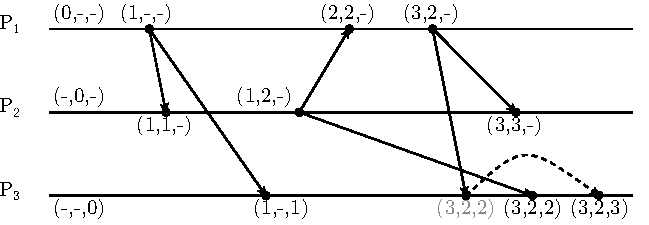
\includegraphics[width=10cm]{kommBeispielCausalBroadcast.pdf}
	\caption[Kommunikation durch Causally Ordered Multicasts]{Ablauf einer Kommunikation zwischen Prozessen, die ausschließlich Causally Ordered Multicasts versenden. Wie man sieht, muss ein Prozess eine Empfangene Nachricht aufheben, bis eine vorher gesendete Nachricht eintrifft.}
	\label{figure:causalbroadcast}
\end{figure}
\FloatBarrier

Der Ablauf des Aufhebens und Verzögerns von gewissen Nachrichten lässt sich durch ein recht einfaches Protokoll darstellen. Dieses ist in Abbildung \ref{figure:causalBroadcastProtocol} dargestellt.

\begin{figure}[ht]
	\centering
	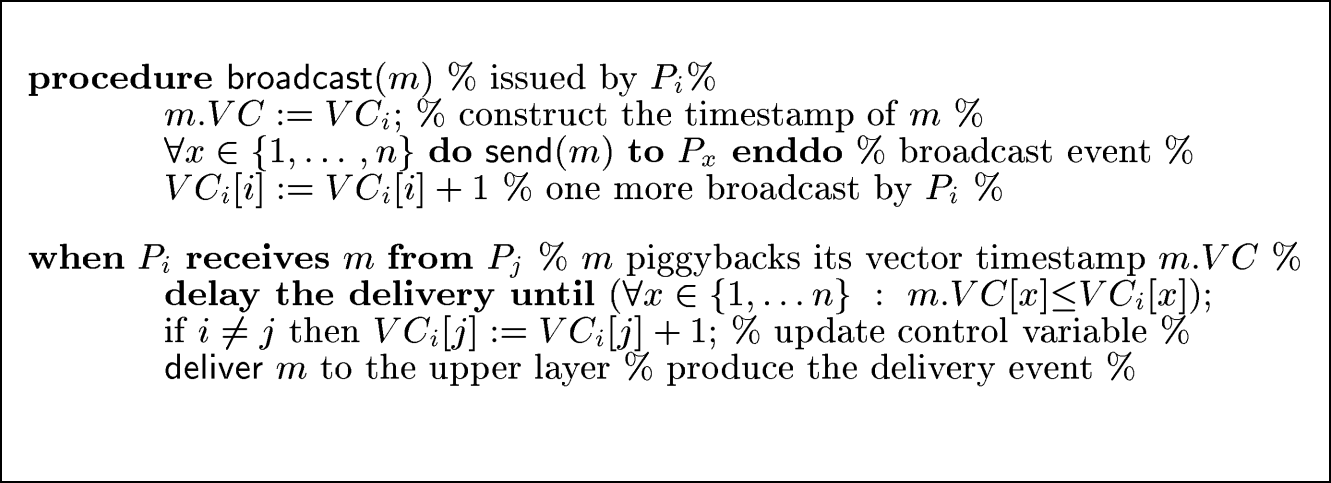
\includegraphics[width=10cm]{causalBroadcastProtocol.png}
	\caption[Protokoll für den Causally Ordered Multicast]{Beschreibung der verarbeitung von Causally Ordered Multicast in Form eines Protokolls.}
	Quelle: \cite{Baldoni:2002:FDC:1435723.1437765}[S. 7, Abbildung 3]
	\label{figure:causalBroadcastProtocol}
\end{figure}
\FloatBarrier

Ausgeschrieben sieht die Funktionalität des Protokolls folgendermaßen aus:

\begin{itemize}
	\item Löst ein Prozess durch ein stattgefundenes Event einen Broadcast aus, so fügt er zunächst seine aktuelle Vektoruhr an die Nachricht des Broadcasts an. Nun sendet er die Nachricht an alle teilnehmenden Prozesse und aktualisiert im letzten Schritt seinen Eintrag in der lokalen Vektoruhr.
	\item Empfängt ein Prozess $P_i$ eine Nachricht m des Prozesses $P_j$, so muss er die Nachricht so lange verzögern, bis die Bedingung $m.VC[x] \le VC_i[x]$ erfüllt ist, also bis die Nachricht ein direkter Nachfolger der Vorherigen ist. Anschließend wird der wert VC[j] inkrementiert, um das Sendeevent des Prozesses $P_j$ zu verzeichnen. Nun kann die Nachricht an die Anwendungsschicht weitergegeben werden.
\end{itemize}

Im Laufe der Kommunikation kann es passieren, dass mehrere nacheinander empfangenen Nachrichten nicht sofort verwendet sondern verzögert werden müssen. Für diesen Fall bietet es sich an, die verzögerten Nachrichten in einer liste zu speichern und bei Eintreffen einer neuen Nachricht alle zunächst zurückgehaltenen nach deren \qq{alter} sortiert zu verarbeiten.

Zu erwähnen ist an dieser Stelle, dass sich die Aktualisierung einer Vektoruhr wie in dem Protokoll beschrieben etwas von der ursprünglichen, rein auf Vektoruhren ausgelegten Vorgehensweise unterscheidet. Wie in Kapitel \ref{prinzipFunktion} unter Satz R1 bis R3 angegeben, inkrementiert ein Node seinen eigenen Eintrag in der lokalen Uhr bei auslösen eines jeden Events. Für Causally Ordered Broadcasts ist dies nur beim verschicken einer Nachricht der Fall, außerdem geschieht dies erst nach dem abschicken. Der Empfänger $P_i$ hat dann die Aufgabe, seine lokale Vektoruhr an der Stelle $VC_i[j]$ zu erhöhen, er ändert bei Causally Ordered Multicasts also den Eintrag eines anderen Prozesses in seiner lokalen Uhr anstatt wie vorher seinen eigenen. Durch diese Anpassung kennt jeder Prozess zu jeder Zeit die Anzahl an abgeschickten Broadcasts an allen Prozessen und kann bei Empfang einer Nachricht sehen, ob alle vorhergehend benötigten Broadcasts bereits eingetroffen sind.
\subsubsection{Weitere Multicast Arten}
%370 Tannenbaum
Neben der Methode, Nachrichten eines Multicasts anhand von deren Kausalität zu ordnen, existieren noch weitere Arten von Multicasts. Diese orientieren sich an den in Kapitel \textit{\ref{chap:ordnung} - \nameref{chap:ordnung}} erläuterten Ordnungsingarten. Neben dem Causally Ordered Multicast sind noch die Arten FIFO-Ordered Multicast sowie Totally Ordered Multicast von Bedeutung. All diese Ordnungsmöglichkeiten werden unter Anderem in \cite{Tanenbaum2007} aufgezeigt.

\subsubsection*{FIFO Ordered Multicast}
Das First-In-First-Out Modell funktioniert ohne Vektoruhren und stellt lediglich sicher, dass die Reihenfolge, welche beim Absenden von Nachrichten aufgetreten ist, von einem empfangenden Prozess eingehalten wird. Hierbei spielt der eventuelle Kausale Zusammenhang der Nachrichten keine Rolle, die Nachrichten erhalten lediglich einen einfachen Zähler für die Absendereihenfolge, welche der Empfänger sicherstellt \cite{Tanenbaum2007}[S. 352].

\subsubsection*{Totally Ordered Multicast}
Eine totale Ordnung lässt sich auf alle anderen Arten von Multicasts anwenden, sei diese völlig ungeordnet, FIFO-geordnet oder kausal geordnet. Bei einer totalen Ordnung wird grundsätzlich gefordert, dass eine Versandreihenfolge, wie auch immer diese geordnet sein mag, bei allen Teilnehmern im System gleich ist \cite{Tanenbaum2007}[S. 352]. Diese Art von Multicast wird auch als Atomic Broadcast bezeichnet. Dieser Name zeigt dabei sehr gut die Eigenschaft, dass entweder alle Nachrichten in der richten Reihenfolge an allen Prozessen versandt werden, oder keine. Der Multicast ist sozusagen atomar und kann nicht geteilt werden \cite{Birman:1987:RCP:7351.7478}[S. 52].

\subsubsection{Umsetzung in C\# auf Basis der Vektoruhr}
Causally Ordered Multicasts wurden als Erweiterung der in Kapitel \ref{vectorClockImpl} beschriebenen Implementierung umgesetzt. In dem gewählten Bank-Szenario sendet ein Bankautomat bei jeder Kontoaktualisierung, also einem Event, einen Broadcast an alle im System vorhandenen Prozesse. Hierbei ist es jedoch egal ob die gesendeten Nachrichten über die Aktualisierung auch ankommen oder nicht beziehungsweise spielt die Reihenfolge des Empfangs für den Sender keine Rolle. Dieses System funktioniert solange, bis ein Prozess einmal eine Aktualisierung zu spät erhält und somit seinen Kontostand nicht entsprechend zum richtigen Zeitpunkt aktualisiert. Um diesem Problem entgegenzuwirken, können Causal Broadcasts verwendet werden.

Als Grundlage dient die in Kapitel \ref{vectorClockImpl} implementierte Vektoruhren-Mechanik. Neben den im vorherigen Abschnitt erwähnten Anpassungen für die Art und Weise, wie lokale Vektoruhren inkrementiert werden, muss für die Umsetzung des Causal Broadcasts ein Speicher für verzögerte Nachrichten eingeführt werden. Dies wurde in Form der Klasse \code{OrderedMessageList} implementiert, welche wie ein Stack mit Nachrichten funktioniert. Um die zeitliche korrekte Reihenfolge der Nachrichten in der Liste zu gewährleisten, werden diese bei jeder Einfüge- oder Entfernoperation anhand von Vergleichen der Vektoruhren sortiert. 

\begin{lstlisting}[label=lst:delayMessage,
language=sharpc,
float=ht,
firstnumber=1,
caption={Auszug aus der Methode \code{HandleCommunicationMessageOrdered()}. Hier wird geprüft, ob schon aufgeschobenen Nachrichten vorhanden sind und ob die angekommende akzeptiert werden kann.}]
 if (delayedMessages.Count == 0) // no delayed messages
 {
 	if (MessageNotAcceptable(msg))   //  delay until vc(x) <= m.vc(x) for all x
 	{
 		delayedMessages.PushItem(msg);   // Put message in queue
 		Console.WriteLine($"    Message {msg.communicationBlock.clock} is to early, delaying...");
 	}
 	else
 	UseMessageOrdered(msg);     // Message ist ok, use it!
 }
 else
 [...]
\end{lstlisting}

Damit ankommende Nachrichten eventuell aufgehoben werden können, muss die Methode \code{HandleCommunicationMessage()} angepasst werden. Diese akzeptiert in der einfachen Vektoruhr-Implementierung alle Nachrichten und verarbeitet deren Inhalt. In der erweiterten Umsetzung, \code{HandleCommunicationMessageOrdered()} genannt, findet vorher eine Überprüfung statt, ob die neue Nachricht akzeptiert wird oder verzögert werden muss. Als Bedingung wird hier geprüft, ob die zu untersuchende Uhr zeitlich gesehen kleiner als die aktuelle lokale Uhr ist. Solange dies der Fall ist, muss die Nachricht aufgeschoben werden. Man kann deshalb sagen, dass ein Node in der Umsetzung des Causally Ordered Multicasts immer auf die nächste fehlende Nachricht wartet und alle neueren Nachrichten als diese aufhebt, bis die passende angekommen ist. Ein Auszug der Methode ist in Listing \ref{lst:delayMessage} abgebildet.

\begin{lstlisting}[label=lst:useMessage,
language=sharpc,
float=ht,
firstnumber=1,
caption={Verarbeitung einer akzeptierten Nachricht.}]
private void UseMessageOrdered(Message msg)
{
	Console.WriteLine($"    Message {msg.communicationBlock.clock} is ok! Using it.");
	this.commLogic.clock.update(msg.communicationBlock.clock);
	this.commLogic.appLogic.balance = msg.communicationBlock.payload.balance;
	if (this.commLogic.clock.getID() != msg.communicationBlock.clock.getID())
	{
		this.commLogic.IncreaseVectorClock(msg.communicationBlock.clock.getID());           // update control variable
		Console.WriteLine($"    Increased clock[{msg.communicationBlock.clock.getID()}]: {this.commLogic.clock}");
	}
}
\end{lstlisting}

Sobald eine Nachricht als akzeptiert eingestuft ist, wird sie durch einen Aufruf der Methode \code{UseMessageOrdered()} verarbeitet und kann nun sozusagen an die Anwendungsschicht weitergegeben werden. Diese Weitergabe geschieht in diesem Beispiel dadurch, dass der lokale Kontostand in der Applikationslogik auf den Stand des sich in der Nachricht befindlichen Kontostandes aktualisiert wird. Listing \ref{lst:useMessage} zeigt die Methode anhand eines Codebeispiels.

In einigen Testläufen des Programms mit drei Prozessen hat sich gezeigt, dass durch die Mechanik des Aufhebens von Nachrichten durch den Broadcast selbst bei mehreren tausend Nachrichten, welche in wenigen Sekunden nacheinander verschickt werden, die korrekte und geforderte Empfangsreihenfolge der Nachrichten anhand der Absendereihenfolge eingehalten werden konnte.

\FloatBarrier

\subsection{Rolle der Anwendungsschicht (Anwendungs-API)}
\label{RolleDerAnwendung}
In diesem Kapitel wird hervorgehoben, welche Funktion die Anwendungsschicht in einem verteilten System einnimmt und wie die Rolle von Vektoruhren im Bezug auf die Verarbeitung und Ordnung von Nachrichten zwischen Prozessen für eine Anwendungs-API aussieht.

\subsubsection{Aufteilung eines verteilten Systems}
Ein verteiltes System kann in seiner Gesamtheit durch verschiedene Schichten dargestellt werden. Dabei stellt jede Schicht nach oben hin zur nächsten eine Abstraktion seiner eigenen Funktionalität dar, welche durch Schnittstellen von der höheren Schicht aufgerufen werden können. Diese Schnittstellen mit samt der angebotenen Funktionalitäten werden auch als Services bezeichnet \cite{Coulouris2011}[S. 52]. In der Literatur finden sich die verschiedensten Modelle zur Einteilung solcher Systeme in einzelne Schichten. Der Zwecke dieser Aufteilung ist es, die Komplexität der einzelnen Aufgabenbereiche zu kapseln und für aufrufende Schichten zu reduzieren. Allgemein gesprochen können die für ein verteiltes System wichtigen Ebenen mit den Schichten 5-7 des ISO-OSI-Referenzmodells verglichen werden \cite{schill12}[S. 40]. Dieses OSI-Modell beschreibt dabei Grundsätzlich, wie eine Kommunikation zwischen unterschiedlichen Computern aufgebaut werden kann. Es wird unter anderem in \cite{ISOOSI} näher beschrieben. Eine solche Aufteilung in Schichten ist in Abbildung \ref{figure:schichtenaufbau} grafisch dargestellt.

 \begin{figure}[ht]
 	\centering
 	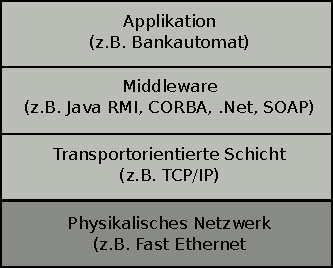
\includegraphics[width=8cm]{VerteiltesSystem.pdf}
 	\caption[Verteiltes System als Schichtemodell]{Aufteilung eines verteilten Systems in einzelne Schichten. Jede Schicht abstrahiert seine Funktionalität zur nächst höheren Schicht und stellt diese durch Schnittstellen bereit.}
 	Quelle: Eigene Darstellung in Anlehnung an \cite{schill12}[S. 41, Abbildung 2.12]
 	\label{figure:schichtenaufbau}
 \end{figure}
 
 Die unterste Schicht kümmert sich um die physikalische Kommunikation der Systeme. Hauptaufgabe der Ebene ist die Bitübertragung auf dem physikalischen Übertragungsweg. In dieser Ebene wird deshalb die gesamte benötigte Hardware abstrahiert, damit sich die oberen Schichten nicht mit dieser beschäftigen müssen. 
 
 Schicht zwei stellt reine Netzwerkfunktionen bereits, damit eine Kommunikation zwischen zwei oder mehreren Prozessen in einem verteilten System überhaupt stattfinden kann. In dieser Schicht befinden sich die Protokolle zur Netzwerkkommunikation, zum Beispiel TCP/IP oder UPD. Hier ist eine Nachricht noch nicht als solche vorhanden, es werden lediglich Byteströme ausgetauscht. Zusammen mit der Schicht für das physikalische Netzwerk abstrahiert diese Schicht von den systemnahen Details \cite{schill12}[S. 40].
 
 Auf dem physikalischen Kommunikationsnetz sowie den Protokollen baut die Middleware auf. Hier befinden sich diejenigen Funktionen, welche eine sinnvolle und korrekte Kommunikation zwischen Prozessen ermöglichen. Ausgehend von den durch die Netzwerkschicht und transportorientierte Schicht angebotenen Funktionen für die physikalische Kommunikation werden nun aus den ankommenden Byteströmen Nachrichten gemacht. In dieser Schicht werden auch alle Arten von logischen Uhren eingeordnet, also auch Vektoruhren. Allgemein abstrahiert diese Schicht die Komplexität des darunterliegenden Netzwerks, der Hardware allgemein sowie des Betriebssystems. Auch die Beschränkung auf eine bestimmte Programmiersprache für die Netzwerkkommunikation wird aufgehoben \cite{Coulouris2011}[S. 17].
 
 Die höchste und damit von den Funktionen her auch am meisten abstrahierte Schicht ist die Applikations- oder Anwendungsschicht. In dieser Schicht befindet sich die Anwendungslogik des Programms, welches auf dem verteilten System läuft. Somit findet in dieser Schicht die eigentliche Logik des erstellten Verteilten Systems statt. In dieser wird entschieden, wie eine ankommende Nachricht behandelt und im Kontext des Einsatzzweckes für das Programm sinnvoll genutzt werden kann. Als Basis dienen hierbei die Nachrichten, welche von der Middleware an die Anwendungsschicht weitergereicht werden. Die Applikationsschicht muss sich also nicht um die physikalische Kommunikation sowie das erzeugen von Nachrichten aus den ankommenden Daten kümmern sonder fokussiert sich voll und ganz auf eine sinnvolle und logische Verwendung der Nachrichten.
 Zusammengefasst ist es das Ziel eines verteilten System, es den Applikationen und damit letzendlich auch dem Benutzer so einfach wie möglich zu machen, auf verteilte Ressourcen zuzugreifen und diese kontrolliert und effizient zu teilen \cite{Tanenbaum2007}[S. 3, Abschnitt 1.2.1]

\subsubsection{Zusammenhang zwischen Vektoruhren und der Anwendungsschicht}
Betrachtet man die Einordnung von Vektoruhren in das Gesamtbild, so fällt auf, dass diese weniger für eine kausale Ordnung von Nachrichten gedacht sind, als für eine Markierung von Zeitpunkten, zu welchen Events in den jeweiligen Prozessen stattgefunden haben \cite{bibid}[S. 15]. Somit stellen Vektoruhren als auch logische Uhren allgemein eine Grundlage für die Anwendungsschicht dar, damit diese ankommende Nachrichten in eine Kausale Ordnung bringen und die Daten der Nachricht verwenden kann. Einen Sonderfall stellt hier der in Kapitel \ref{causallyorderedmulticast} vorgestellte Causally Ordered Multicast dar, bei welchem eine gleiche Reihenfolge zwischen Absenden und Empfang von aufeinander folgenden Broadcasts auf der Ebene der Vektoruhren gefordert wird.

Wird durch die Middleware eine Nachricht empfangen, so gibt diese die Nachricht nach Aktualisierung der Vektoruhr an die Anwendungsschicht weiter. Es liegt nun an der Anwendungslogik, die Nachricht mit samt der kausalen Information, welche durch die Vektoruhr generiert wird, zu verarbeiten. 

Bei der Ordnung der Nachrichten auf Anwendungsebene können diese durch die Anwendungs-API markiert werden. Dadurch könnte eine Logik bei empfangenen Nachrichten, welche als alt markiert wurden entscheiden, ob diese direkt gelöscht werden sollen. Auch wichtig ist hierbei die Art der Daten, welche zwischen den verteilten Prozessen im System verarbeitet werden. So macht es einen großen Unterschied für die Anwendung, ob zwei Prozesse zeitgleich im Sinne von Events das selbe Datum bearbeiten oder auf unterschiedlichen Daten arbeiten. Eine Anwendung könnte demnach in der Nachricht gesondert Markieren, welches Datum geändert wurde, sodass in diesem Fall eventuell ein Konflikt auf der Vektoruhr-Ebene tatsächlich für das auszuführende Programm keine Auswirkungen hätte und somit ignoriert werden kann.



TODO: Ordnung hängt von Anwendungsfall ab